\section{SCELTA DEI COLORI }
I \textbf{colori} principali del sito saranno:
\\
%ho messo colori a caso dopo i primi due
 
\begin{tikzpicture}
  \fill[verdino, draw=black] (0,0) rectangle (3,3);
  \node[text width=0.7\textwidth, align=justify, anchor=west] at (3.2,1.5) {\textcolor{verdino}{00AE46:} Il colore 00ae46 è un verde vivace che evoca natura e vitalità. Perfetto per un sito che vende dinosauri, offre un legame con l'habitat preistorico dei dinosauri, suggerisce crescita e rinascita, fornisce un contrasto visivo accattivante e attrae il pubblico giovane.};
\end{tikzpicture}
\\

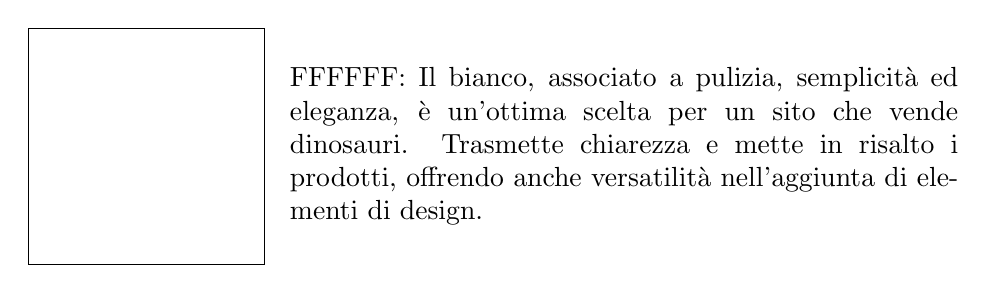
\begin{tikzpicture}
\fill[white, draw=black] (0,0) rectangle (3,3);
\node[text width=0.7\textwidth, align=justify, anchor=west] at (3.2,1.5) {\textcolor{black}{FFFFFF:} Il bianco, associato a pulizia, semplicità ed eleganza, è un'ottima scelta per un sito che vende dinosauri. Trasmette chiarezza e mette in risalto i prodotti, offrendo anche versatilità nell'aggiunta di elementi di design.};
\end{tikzpicture}
\\

\begin{comment}
\begin{tikzpicture}
    \fill[biancosporco, draw=black] (0,0) rectangle (3,3);
    \node[text width=0.7\textwidth, align=justify, anchor=west] at (3.2,1.5) {\textcolor{black}{F5F5F5:} };
    \end{tikzpicture}    
\end{comment}
